\documentclass[a4paper,14pt]{article}
\usepackage{amsmath}
\usepackage[T2A]{fontenc}
\usepackage[utf8]{inputenc} 
\usepackage{graphicx}
\graphicspath{{img/}}
\DeclareGraphicsExtensions{.png,.jpg}
\usepackage{multicol}

\usepackage[russian]{babel} % правила переноса
\usepackage[left=2cm,right=2cm,
top=2cm,bottom=2cm,bindingoffset=0cm]{geometry} % для изменения размеров полей документа
\usepackage{commath}
\usepackage{listings}
\lstset{
      language=Matlab,
      inputpath=m,
      extendedchars=true,
      keepspaces=true,
      breaklines=true,
      basicstyle=\small\ttfamily,
      literate={а}{{\selectfont\char224}}1
               {б}{{\selectfont\char225}}1
               {в}{{\selectfont\char226}}1
               {г}{{\selectfont\char227}}1
               {д}{{\selectfont\char228}}1
               {е}{{\selectfont\char229}}1
               {ё}{{\"e}}1
               {ж}{{\selectfont\char230}}1
               {з}{{\selectfont\char231}}1
               {и}{{\selectfont\char232}}1
               {й}{{\selectfont\char233}}1
               {к}{{\selectfont\char234}}1
               {л}{{\selectfont\char235}}1
               {м}{{\selectfont\char236}}1
               {н}{{\selectfont\char237}}1
               {о}{{\selectfont\char238}}1
               {п}{{\selectfont\char239}}1
               {р}{{\selectfont\char240}}1
               {с}{{\selectfont\char241}}1
               {т}{{\selectfont\char242}}1
               {у}{{\selectfont\char243}}1
               {ф}{{\selectfont\char244}}1
               {х}{{\selectfont\char245}}1
               {ц}{{\selectfont\char246}}1
               {ч}{{\selectfont\char247}}1
               {ш}{{\selectfont\char248}}1
               {щ}{{\selectfont\char249}}1
               {ъ}{{\selectfont\char250}}1
               {ы}{{\selectfont\char251}}1
               {ь}{{\selectfont\char252}}1
               {э}{{\selectfont\char253}}1
               {ю}{{\selectfont\char254}}1
               {я}{{\selectfont\char255}}1
               {А}{{\selectfont\char192}}1
               {Б}{{\selectfont\char193}}1
               {В}{{\selectfont\char194}}1
               {Г}{{\selectfont\char195}}1
               {Д}{{\selectfont\char196}}1
               {Е}{{\selectfont\char197}}1
               {Ё}{{\"E}}1
               {Ж}{{\selectfont\char198}}1
               {З}{{\selectfont\char199}}1
               {И}{{\selectfont\char200}}1
               {Й}{{\selectfont\char201}}1
               {К}{{\selectfont\char202}}1
               {Л}{{\selectfont\char203}}1
               {М}{{\selectfont\char204}}1
               {Н}{{\selectfont\char205}}1
               {О}{{\selectfont\char206}}1
               {П}{{\selectfont\char207}}1
               {Р}{{\selectfont\char208}}1
               {С}{{\selectfont\char209}}1
               {Т}{{\selectfont\char210}}1
               {У}{{\selectfont\char211}}1
               {Ф}{{\selectfont\char212}}1
               {Х}{{\selectfont\char213}}1
               {Ц}{{\selectfont\char214}}1
               {Ч}{{\selectfont\char215}}1
               {Ш}{{\selectfont\char216}}1
               {Щ}{{\selectfont\char217}}1
               {Ъ}{{\selectfont\char218}}1
               {Ы}{{\selectfont\char219}}1
               {Ь}{{\selectfont\char220}}1
               {Э}{{\selectfont\char221}}1
               {Ю}{{\selectfont\char222}}1
               {Я}{{\selectfont\char223}}1
               }
\usepackage[framed,numbered,autolinebreaks,useliterate]{mcode}

\begin{document}

%%%%%%%%%%%%%%%%%%%%%% Титульный лист %%%%%%%%%%%%%%%%%%%%%%

\begin{titlepage}
	\newpage
	
	\begin{center}
		Санкт-Петербургский политехнический 
		университет Петра Великого \\
		\vspace{0.2cm}
		Институт компьютерных наук и технологий\\*
%		\hrulefill
	\end{center}
	
	\vspace{10em}
	
	\begin{center}
		 Отчёт по лабораторной работе № 6
	\end{center}
	
	\vspace{2.5em}

	\vspace{6em}
	\flushleft{Выполнила студентка гр.33501/3: Ивашкевич О.А.}

	\flushleft{Преподаватель: Богач Н.В.}
	\vspace{\fill}
	
	\begin{center}
		Санкт-Петербург
		
		 2017
	\end{center}
	
\end{titlepage}

\tableofcontents

\newpage

\part*{Лабораторная работа №6. Цифровая модуляция}
\setcounter {section}{0}
\setcounter {equation}{0}
\setcounter {figure}{0}
\section{Цель работы}
\hspace{0,5cm}   Изучение методов модуляции цифровых сигналов.
\section{Постановка задачи}	
\hspace{0,5cm}Получить сигналы BPSK, PSK, OQPSK, genQAM, MSK, M-FSK модуляторов.\\
	
Построить их сигнальные созвездия.\\
	
Провести сравнение изученных методов модуляции цифровых сигналов.\\
	
\section{Теоретическое обоснование}

В настоящее время большая часть информации, передаваемой по разнообразным каналам связи, существуют в цифровом виде. Это означает, что передаче подлежит не непрерывный модулирующий сигнал, а последовательность целых чисел, которые могут принимать значения из некоторого фиксированного конечного множества. Для передачи таких сигналов возможно использование методов цифровой модуляции (манипуляции). \\
Типичный подход при осуществлении передачи дискретной последовательность символов состоит в следующем. Каждому значению сопоставляется набор значений параметров несущего колебания. Несущим колебанием может быть сигнал произвольной формы, но чаще используют гармонические колебания. Цифровые символы передаются с некоторым периодом Т, в течение которого значение не меняется, а значит, не меняются и параметры несущего сигнала. По типу параметров, значения которых кодируют входные символы, выделяют амплитудную, частотную, фазовую и квадратурную манипуляцию.

\subsection{Частотная манипуляция}

При частотной манипуляции (frequency shift keying - FSK) каждому возможному значению передаваемого символа сопоставляется своя частота. В течении каждого символьного интервала передается гармоническое колебание с частотой, соответствующей текущему символу. В общем случае при переходе от одного символа к другому происходит скачок фазы несущего колебания. Это приводит к появлению в спектре сигнала скачков на частотах, кратных символьной скорости. Для борьбы с ними можно использовать частотную манипуляцию с непрерывной фазовой функцией.
При этом формируется линейно без скачков за счет интегрирования, а передаваемые символы управляют скоростью ее изменения.\\
 Демодуляция производится корреляционным методом. Т.к. разным значениям отсчетов соответствует своя частота, можно рассчитать взаимную корреляцию полученного сигнала с эталонными значениями для каждой из частот и выбрать ту, с которой корреляция максимальна.
Для повышения помехоустойчивости частоты желательно, чтобы посылки, соответствующие разными символами, были некоррелированными. Для реализации требования некоррелированности должны быть выполненны следующие условия:

$$
\Delta \omega_{min} = \frac{\pi}{T}, \Delta f_{min} = \frac{1}{2T}=\frac{f_T}{2}
$$, где $ frac{f_T} $ - символьная скорость.

Двухпозиционная ЧМн, частоты которой выбраны согласно формуле получила название минимальной частотной манипуляции.

\subsection{Квадратурная манипуляция}

Амплитудная и фазовая манипуляция являются частным случаем квадратурной манипуляции. При квадратурной манипуляции несущее колебание составляется по следующей формуле:
$$
C_k \rightarrow (a_k, b_k), s(t) = a_k\cos(\omega_0 t)+ b_k \sin(\omega_0 t), kT \leq t < (k+1)T
$$
С помощью тригонометрических преобразований эту форму можно привести к виду 
$$
s(t) = A_k \cos(\omega_0 t+\phi_k)
$$
В этой форме сигнал удобно расматривать как комплексное число $A_k \exp(j\phi_k)$.  Совокупность этих комплексных чисел для всех возможных значениц дискретного символа называется сигнальным созвездием. Для возможности сравнения эффективности различных видов модуляции сигнальное созвездие строится для нормированных значений амплитуды и всегда расположено внутри единичной окружности на комплексной плоскости. При этом чем больше расстояние между точками созвездия, тем больше надежность манипуляции. Также квадратурная манипуляция обеспечивает большую помехоустойчивость, чем АМн и ФМн.

Деомодулируется сигнал с квадратурной манипуляцией так же, как и в случае с аналоговой квадратурной модуляции - сигнал умножается на два несущих колебания, сдвинутых по фазе относительно друг друга на 90 градусов, а результаты умножения пропускаются через ФНЧ.

\section{Ход работы}

С помощью Matlab получим сигнальные созвездия сигналов BPSK, PSK, OQPSK, genQAM и MSK модуляторов:

\subsection{BPSK}

\begin{lstlisting}
%% BPSK 
M = 2;
s = randint(1, 1000, [0 M-1]); %digital message
ph = -pi/16;
bpsk = pskmod(s, M, ph); % modulation
h = scatterplot(bpsk, 1, 0, 'o'); % output constellation
grid on; hold on;
bpsk_err = bpsk+randerr(1,1000,100); % signal with errors
scatterplot(bpsk_err, 1, 0,'r.', h);
title('BPSK');
hold off;
msg = pskdemod(bpsk_err, M, ph);
[Num,Rat] = symerr(s, msg)
\end{lstlisting}

\begin{figure}[bh]
\noindent\centering{
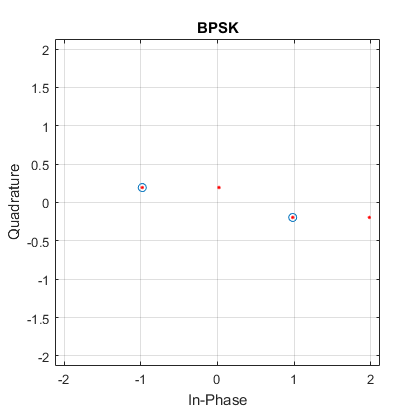
\includegraphics[width=100mm]{BPSK}}
\caption{Сигнальное созвездие BPSK}
\label{figCurves}
\end{figure}
Результат: $Num=0, Rat=0$.

\newpage
\subsection{PSK}

\begin{lstlisting}
%%PSK
M = 8;
s = randint(1000, 1, [0 M-1]); % digital message
ph = pi/4;
psk = pskmod(s, M, ph); % modulation
h = scatterplot(psk, 1, 0, 'o'); % output constellation
grid on;
hold on;
err = randerr(1, 1000, 100)'; % massiv of errors, 100 pcs
psk_err = psk+err; % signal with errors
scatterplot(psk_err, 1, 0, 'r.', h);
title('8-PSK');
hold off;
msg = pskdemod(psk_err, M, ph);
[Num,Rat] = symerr(s, msg)
\end{lstlisting}

\begin{figure}[bh]
\noindent\centering{
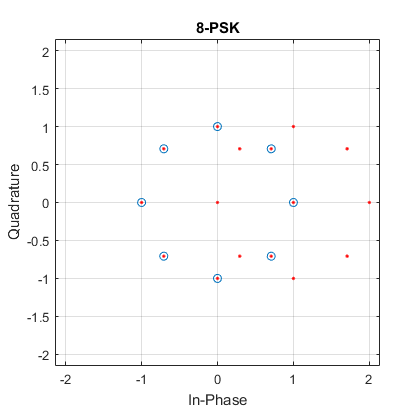
\includegraphics[width=100mm]{PSK}}
\caption{Сигнальное созвездие PSK}
\label{figCurves}
\end{figure}
Результат: $Num=73, Rat=0.073$.

\newpage

\subsection{OQPSK}

\begin{lstlisting}
%% OQPSK
M = 4;
s = randint(1000, 1, [0 M-1]); % digital message
ph = -pi/8;
oqpsk = oqpskmod(s, ph); % modulation
h = scatterplot(oqpsk, 2, 1, 'o'); % output constellation
grid on;
hold on;
err = randerr(1, 2*1000, 2*100)'; % massiv of errors, 100 pcs
oqpsk_err = oqpsk+[err; 0]; % signal with errors
scatterplot(oqpsk_err, 2, 1, 'r.', h);
title('OQPSK');
hold off;
msg = oqpskdemod(oqpsk_err, ph);
[Num,Rat] = symerr(s, msg)
\end{lstlisting}

\begin{figure}[bh]
\noindent\centering{
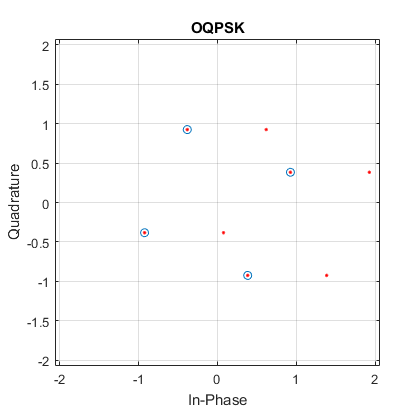
\includegraphics[width=100mm]{OQPSK}}
\caption{Сигнальное созвездие OQPSK}
\label{figCurves}
\end{figure}
Результат: $Num=4, Rat=0.004$.

\newpage

\subsection{genQAM}
\begin{lstlisting}
%% genQAM
c = [2i -5i -5 5 3.5-2.5i -3.5-2.5i -4.75+2i +4.75+2i -4+3.25i +4+3.25i -3+4i 3+4i -1.7+3.5i 1.7+3.5i -0.8+2.75i 0.8+2.75i];
M = length(c); % 16

s = randint(1000, 1, [0 M-1]);
modData = genqammod(s, c);
h = scatterplot(modData, 1, 0, 'o');
grid on;
hold on;
rxSig = modData + randerr(1, 1000, 100)';
scatterplot(rxSig, 1, 0, 'r.', h);
title('QAM');
hold off;
z = genqamdemod(rxSig, c);
[Num,Rat] = symerr(s, z)
\end{lstlisting}

\begin{figure}[bh]
\noindent\centering{
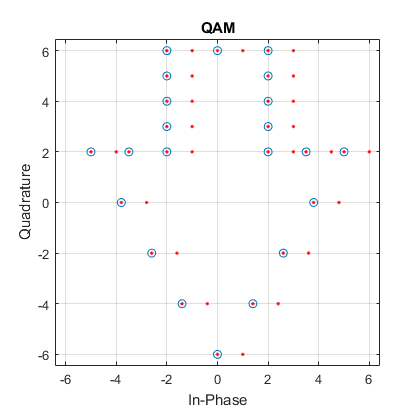
\includegraphics[width=100mm]{QAM}}
\caption{Сигнальное созвездие genQAM}
\label{figCurves}
\end{figure}
Результат: $Num=27, Rat=0.027$.

\newpage

\subsection{MSK}
\begin{lstlisting}
%% MSK 
s = randint(1000, 1, [0 1]);
ph = pi/2;
msk = mskmod(s, 8, [], ph);
h = scatterplot(msk, 8, 0, 'o'); % output constellation
grid on;
hold on;
msk_err = msk-randerr(1, 8*1000, 8*100)'; % signal with errors
scatterplot(msk_err, 8, 0, 'r.', h);
title('MSK');
hold off;
msg = mskdemod(msk_err, 8, [], ph);
[Num,Rat] = symerr(s, msg)
\end{lstlisting}

\begin{figure}[bh]
\noindent\centering{
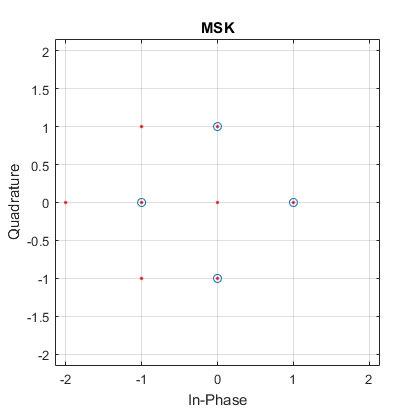
\includegraphics[width=100mm]{MSK}}
\caption{Сигнальное созвездие MSK}
\label{figCurves}
\end{figure}
Результат: $Num=0, Rat=0.0$.



\section{Выводы}
\hspace{0,5cm} 
По итогам работы было получено, что наибольшая ошибка в QAM модуляторе, которая обуславливается большим количеством закодированным символов, по причине, маленького расстояния Хэмминга между ближайшими точками созвездия на комплексной плоскости. Однако, скорость QAM большая. PSK сигнал демодулирован без ошибок. При демодуляции сигнала MSK получено меньше ошибок, так как в нем закодировано меньше символов, чем в QAM.
\end{document}